\documentclass[a4paper,12pt,abstracton]{scrartcl}
\usepackage[utf8]{inputenc}
\usepackage{float}
\usepackage{amsmath}
\usepackage{amssymb}
\usepackage{pifont}% http://ctan.org/pkg/pifont
\usepackage[font=small,labelfont=bf]{caption}
\usepackage{graphicx}
%\usepackage{dirtytalk}
\usepackage{multicol}
\usepackage{booktabs}
\usepackage{colortbl}
\usepackage{appendix}
\usepackage{nomencl}
\usepackage{lmodern}
\usepackage[nottoc]{tocbibind}
\usepackage{xcolor}
%\graphicspath{images/}
\usepackage[margin = 3cm]{geometry}
\usepackage{ragged2e} % good alignment
\usepackage{hyperref}
\usepackage{siunitx} % Provides the \SI{}{} and \si{} command for typesetting SI units
\hypersetup{colorlinks=true,
    linkcolor=blue,
    filecolor=magenta,      
    urlcolor=cyan, 
    citecolor=gray}

%\DeclareGraphicsExtensions{.png,.pdf} % low-res (work in progress)
%\DeclareGraphicsExtensions{.pdf,.png}  % high-res (final draft)
%\setlength\parindent{0pt} % Removes all indentation from paragraphs
%\bibliographystyle{unstr}
\setlength\parindent{0pt}
\setlength{\parskip}{0.3em}
\newcommand{\xmark}{\ding{55}}

\renewcommand{\nomname}{List of Symbols}
\renewcommand{\nompreamble}{The following list explains the symbols used within the body of the report.}

\usepackage{etoolbox}
\renewcommand\nomgroup[1]{%
  \item[\bfseries
  \ifstrequal{#1}{E}{Experimental Equipment}{%
  \ifstrequal{#1}{C}{Computational Methods}{%
  \ifstrequal{#1}{T}{Theoretical Concepts}{
  \ifstrequal{#1}{P}{Physical Constants}{}}}}%
]}


\subject{CMP Lab Report} % Matter Physics, Physics, Chemical Physics ?
\title{Zeeman Effect}
\author{Group B9\footnote{Pietro Monticone , Claudio Moroni , Alberto Mosso , Riccardo Valperga.}}

\renewcommand{\listfigurename}{Plots}
\renewcommand{\listtablename}{Tables}
\renewcommand{\nomname}{Nomenclature}


\begin{document}
\maketitle
\makenomenclature
\begin{abstract}
This experiment examined the normal and anomalous Zeeman effect with the aim of calculating the Bohr magneton by fitting the energy gap between spectral lines of a cadmium lampas surrounded in a magnetic field, as a function of the magnitude of the magnetic field. In the first section, the magnet calibration and the procedure adopted to test the uniformity of the magnetic field, are described. Regarding the former, we expected the magnetic field to vary almost linearly with the current since we worked with soft ferromagnets. For what concern the latter, we have made sure that for small movement in the region occupied by the cadmium lamp, the magnitude of the magnetic field did not vary substantially. Lastly, with a CCD camera and with the help of a polarizing filters and a retarding lamina, several images of the splitted spectral lines have been taken in several different configurations. The configurations depended on the longitudinal or traversal orientation of the magnets compared to the optical axe of the experimental apparatus; and the different configuration of the polarizing filters placed along the light path. The results are four estimates of the Bohr magneton that has been compared with the theoretical value.
\end{abstract}
\clearpage
\tableofcontents
%\listoffigures
%\listoftables

\mbox{
\nomenclature[C]{MC}{Monte Carlo}
\nomenclature[E]{CB}{Cosmic Box}
\nomenclature[P]{$m_e$}{Electronic Mass}
\nomenclature[P]{$e$}{Electronic Charge}
\nomenclature[T]{$V_{disc}$}{Discriminator Voltage}
}
\newpage
\section{Experimental Apparata and Procedures}
\subsection{B-I curve retrival and Magnetic Field Uniformity check}
\subsubsection{Experimental apparatus}
The apparatus is composed of two ferromagnetic-core electromagnetic expansions connected to a current generator, an amperometer ***insert amperometer type NO*** and a magnetometer ***insert magnetomenter name NO***.
\subsubsection{Procedure}
The first goal is to extrapolate from a series of measurements a B(I) relation, where B is the magnetic field and I the current flowing through the expansions. 
Using the following circuit \footnote{The capacity C is large and it is there for safety reasons, should one accidentally induce a short-circuit.}
\begin{figure}[H]
\begin{center}
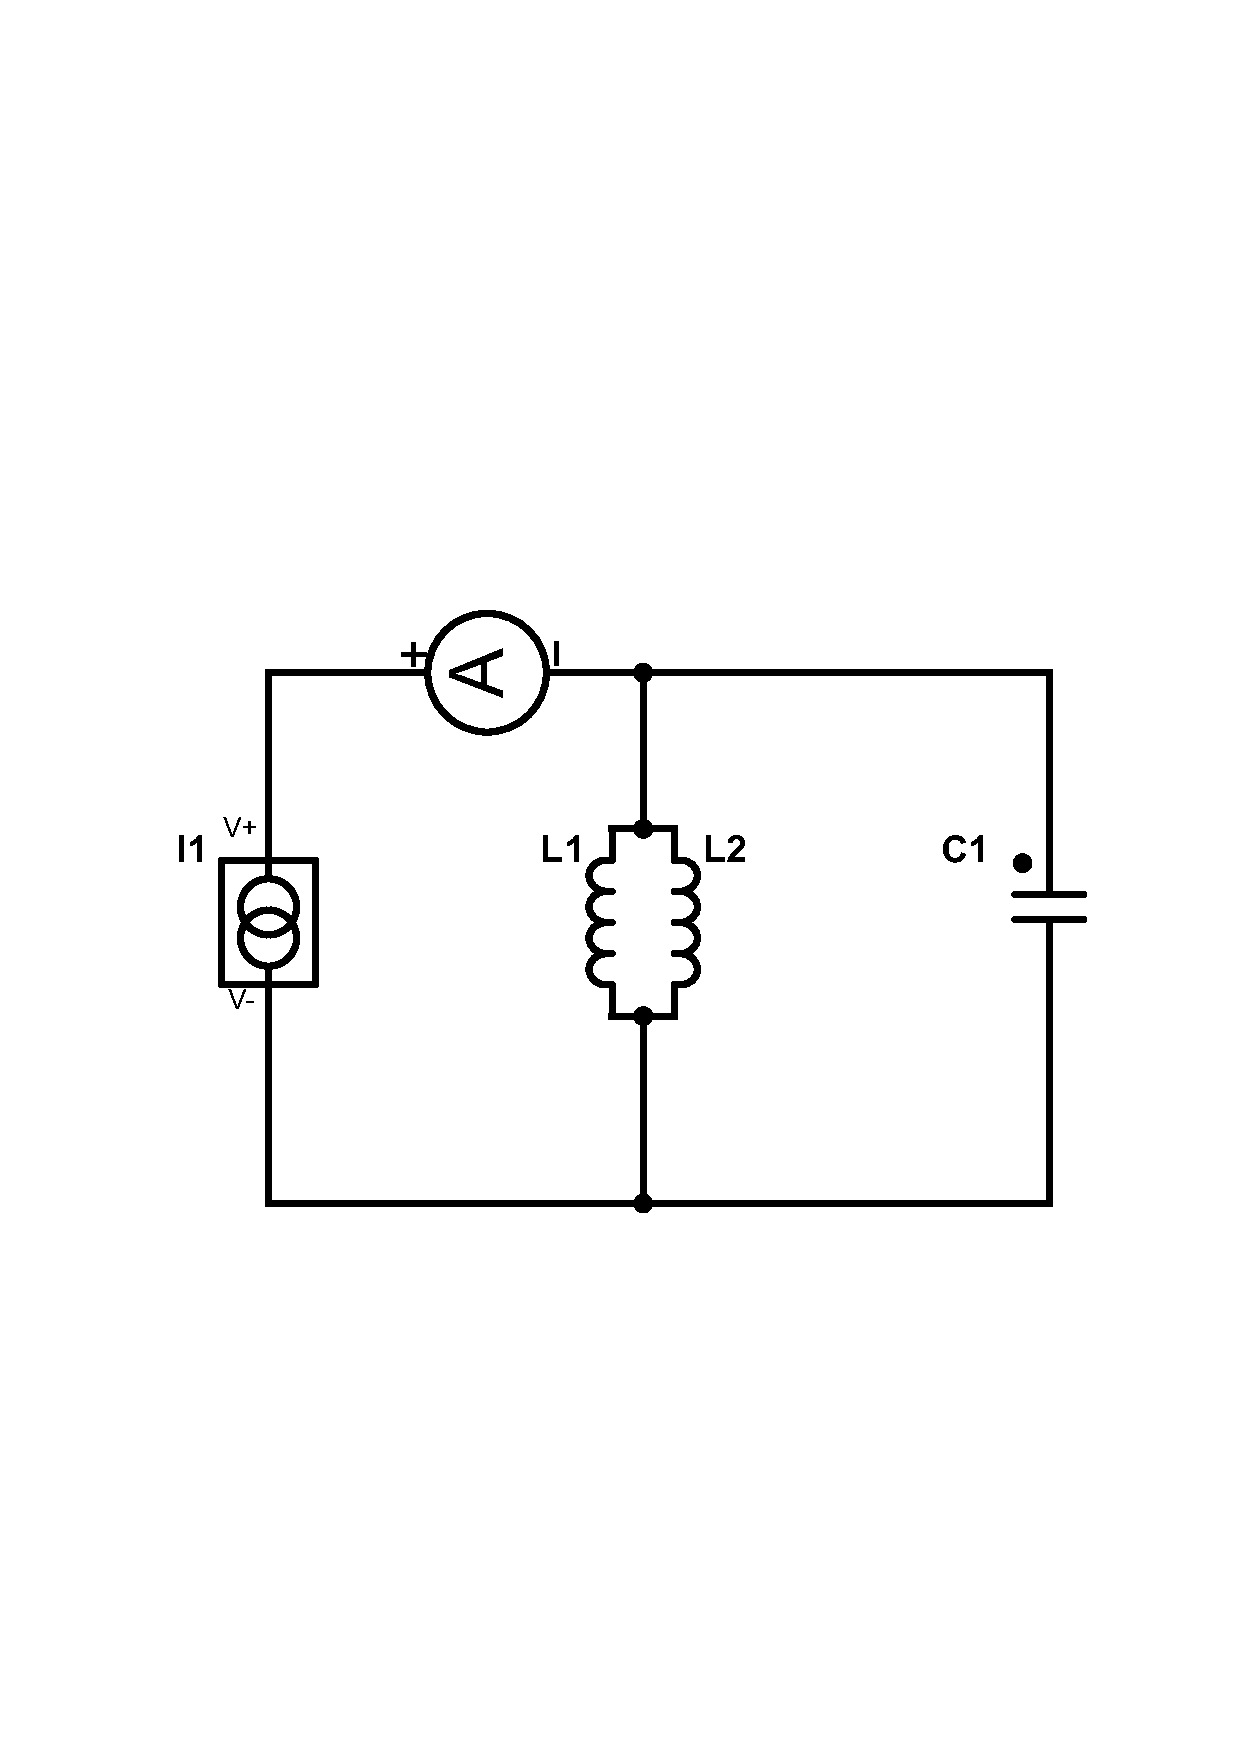
\includegraphics[trim=3cm 8cm 2.5cm 10cm,clip,width=7.5cm,keepaspectratio]{circuito1.pdf} 
\caption{http://www.partsim.com/simulator (vi piace?)}
\end{center} 
\end{figure}
The current has been varied about 1A stepwise (read on the amperometer) and the magnetic field measured in the middle of the expansions. The current sequences $0A \longrightarrow 10A \longrightarrow 0A \longrightarrow 10A$ were performed.
Then, by choosing a specific current value, the magnetic field has been measured at different positions between the expansions. This was needed on order to assign a more precise uncertainty to the values of B.
\subsection{Zeemann Effect}
\subsubsection{Experimental apparatus}
An optical bench featuring a cadmium spectroscopic light source inserted between the electromagnets discussed above, a diaphragm, a Fabry-Perot interferometer, a wavelength filter, a polarizer, a retarding lamina and A CCD camera has been used. A particular wavelength $\lambda$ interval of the light coming from the source was selected via the filter before entering the interferometer. Because of the functioning of the Fabry-Perot interferometer an input wavelength is diffracted in a series of circular spectral lines. As the filter acts on an interval of $\lambda$,we could observe the splitting of a wavelength into two/three (normal logitudinal/transverse effect : see \ref{subsec:1}) or six/nine (longitudinal/transverse anomalous), without dealing with extra lines. The Fabry-Perot interferometer main characteristic is the following:\newline
defined $$\delta = r^2_{n,a}-r^2_{n,b}$$ and $$\Delta = r^2_{n+1,a}-r^2_{n,a}$$  where $r_{n,a}$ is the radius of the n-th order spectral line corresponding to the wavelength a, we have that $\delta$ and $\Delta$ are approximately constant with respect to n and $\lambda$ when $a\simeq b$. Moreover, by geometric means, one finds that 
\begin{equation} \label{eq:1}
\Delta E  = \frac{hc}{2\mu t} \frac{\delta}{\Delta}
\end{equation}
 where $\mu$ is the refracive index of the interferometer and t is its thickness. So one is able to calculate $\Delta E$ from the images acquired form the CCD camera.
\subsubsection{Procedure} \label{subsec:1}
The experimental procedures followed to observe the normal zeemann effect and the anomalous one were similar. The magnets could be rotated, giving rise to the possibility of perpendicular and longitudinal configurations (orientations are referred to the optical bench axis). When considering the former, output light was linearly polarized (one could choose to observe the 2 linear polarizations by rotating the axis of the polarizer, no retarding lamina needed); the latter returned circularly polarized light: the lamina was used in combinations with the polarizer. It is to be said that in longitudinal configuration a light component, namely the one that would have polarization parallel to propagation direction, disappeared.\newline
Wavelength $643.847 nm$ corresponding to $3 ^{1}D_{2} \longrightarrow 2 ^{1}P_{1}$  transition was selected to observe normal zeeman effect, while wavelength $508.588 nm$ corresponding to $3 ^3S_1 \longrightarrow 2 ^3P_2$ was chosen to observe the anomalous one. \newline
At each value of the current flowing through the electromagnets three snapshots (diffractograms) of the CCD were taken: the first depicting all lines, the second and the third were retrieved after inserting the polarizer and selecting one polarization and the other. This was executed for both the normal and anomalous settings, in transverse and longitudinal configurations.\newline
Thus for each value of current (i.e. for each value of magnetic field extrapolated from the B-I curve one got before) we had many values of $\delta \text{ and } \Delta $ (all we could get form the three CCD snapshots), whose averages were to be used to get $\Delta E$ from \ref{eq:1}. Measures of $\delta$ and $\Delta$ were taken on diffractograms using Motic Images Plus 3.0 software.
Thus one ends up with four linear fits of $\Delta E \text{ vs } B$, from which we could get four estimates of $\mu_B$, that were then compared, averaged and compared with the theoretical value. According to $g_{jls} , \; m_l \text{ and } m_j$ values, we used $\Delta E = \mu_B B$ to fit normal zeemann effect data, and $\Delta E =\frac{1}{2} \mu_B B$ for the anomalous one.
%\bibliographystyle{unsrt}
%\bibliography{biblio}
\end{document}
